% Elsevier LaTeX template for Energy Research & Social Science
% Overleaf: upload the whole paper/ folder (main.tex + figures/). Compiler: pdfLaTeX.
% Every number in this file comes from results/headline_stats.md and results/extra_analysis.md,
% produced by scripts/headline_stats.py and scripts/extra_analysis.py.
% Figures come from scripts/paper_figures.py.
% Items in blue \note{...} are notes for the authors: things still to confirm, add or decide.
% The graphical abstract was removed on purpose: it is the last step, once the paper is in good shape.
\documentclass[preprint,12pt,number]{elsarticle}

\usepackage{amssymb}
\usepackage{amsmath}
\usepackage{graphicx}
\usepackage{booktabs}
\usepackage{multirow}
\usepackage{float}
\usepackage{xcolor}
\usepackage{hyperref}

\graphicspath{{figures/}}
% Notes for the authors. Before submission, resolve them all or redefine \note to print nothing.
\newcommand{\note}[1]{\textcolor{blue}{[NOTE: #1]}}

\journal{Energy Research \& Social Science}

\begin{document}

\begin{frontmatter}

\title{Diversity Awareness and Representation in Energy Publications}

\author[imp]{Azhar Nurgaliyeva}
\author[imp]{Anandha Gopalan}
\author[imp]{Anna Korre}

\affiliation[imp]{organization={Imperial College London},
            city={London},
            country={United Kingdom}}
% \note{author order, corresponding author, departments}

\begin{abstract}
The energy transition depends on a research workforce that draws on all available talent, yet women remain under-represented in energy research and there is little field-specific evidence on where the gaps arise. Existing bibliometric studies mostly report aggregate figures for science and engineering and rarely compare energy sub-fields or countries. This paper quantifies gender representation, its change over time and its relationship with research impact and seniority in energy publications. We analyse 15,730 articles (17,148 article-country records) published between 2010 and 2025 in six Elsevier journals spanning energy science, engineering and policy, with authors affiliated with eight countries: the UK, France, Germany, Switzerland, the USA, Canada, South Africa and Singapore. Bibliographic records were enriched with citation counts, alternative metrics and author h-indices, and first-author gender was inferred from names. We find that women are 26.8\% of first authors, ranging from 22.2\% to 34.4\% across journals and from 23.4\% to 32.2\% across countries. The share has risen by about 0.37 percentage points per year, most clearly in \textit{Solar Energy} and \textit{Energy Policy}. The raw citation gap of 7.13\% in favour of men is not statistically significant and disappears once publication year, journal and country are accounted for, and women are equally represented among the most highly cited articles. The sharpest gradient is in seniority: the female share falls from 31\% among first authors with an h-index of 0-2 to 13\% among those above 40, and women are less likely to publish repeatedly as first author. These results suggest that the main inequality in energy research lies in participation and progression rather than in how women's work is received, which points to retention and career development as priorities for equity, diversity and inclusion efforts. We also show that estimates of female representation, and the ranking of some countries, are highly sensitive to the confidence threshold of the gender classifier, an important caveat for bibliometric equity studies.
\end{abstract}

% Elsevier highlights: max 85 characters each, including spaces.
\begin{highlights}
\item Women are 26.8\% of first authors across six Elsevier energy journals
\item Female first authorship rose by about 0.37 points per year over 2010-2024
\item Female share falls from 31\% of junior to 13\% of the most senior first authors
\item No citation penalty for female first authors after adjusting for context
\item Female share estimates depend strongly on the gender-classifier threshold
\end{highlights}

\begin{keyword}
energy research \sep gender equity \sep bibliometrics \sep authorship patterns \sep research impact
\end{keyword}

\end{frontmatter}

%===========================================================
\section{Introduction}
%===========================================================

\subsection{Why diversity matters in energy research}

The global energy transition requires diverse perspectives to address complex technical, social and policy challenges \citep{UNESCO2017,Elsevier2020}. Decisions about which technologies are developed, how they are deployed and who benefits from them are shaped by the people who carry out and lead energy research. A research community that draws on a narrow part of the population risks narrower research agendas, blind spots in the design of technologies and policies, and a loss of talent at a time when the sector needs to grow quickly.

Gender is the dimension of diversity for which the evidence is most extensive, and it shows a persistent imbalance. Women remain a minority of the energy workforce, particularly in technical, research and leadership roles \citep{Pearl-Martinez2016,IRENA2019}. The imbalance is global, although its size differs between countries and between parts of the energy sector \citep{IRENA2019}. \note{expand why gender matters globally, e.g.\ IEA and IRENA workforce figures by region, links to energy access and to the Sustainable Development Goals on gender equality and clean energy}

This study was carried out within IGNITE Network+, a network funded by the UK Engineering and Physical Sciences Research Council that aims to make the energy research community more diverse and inclusive by identifying barriers at each career stage and testing ways to remove them \note{add a citation or URL for IGNITE Network+ and confirm the wording}. One of the network's premises is that under-representation results from systemic barriers rather than from a lack of talent, and that such barriers can only be addressed if they are first made visible with data. Publications are one of the few sources that allow this to be done consistently across countries, research fields and time.

\subsection{Gender gaps in scientific publishing}

Large-scale bibliometric studies have documented gender gaps in authorship across the sciences. Women are a minority of authors worldwide and are less likely to hold the first and last author positions that signal leadership of the work \citep{Lariviere2013,West2013}. The gap is closing slowly, and at current rates parity is decades away in fields such as physics, computer science and engineering \citep{Holman2018}. Evidence on research impact is more mixed. Some studies report that papers led by women receive fewer citations \citep{Lariviere2013}, whereas career-level analyses suggest that differences in productivity and impact are largely explained by differences in career length and drop-out rates, with men and women publishing at similar annual rates and receiving similar impact for the same body of work \citep{Huang2020}. This distinction matters for policy: a citation penalty would point to bias in how work is received, whereas a career-length effect would point to retention and progression.

Much less is known about energy research specifically. An analysis of 15 years of articles in three leading energy journals found that fewer than one in six authors could be identified as women \citep{Sovacool2014}. Most later evidence concerns the energy workforce or energy policy rather than research publications \citep{Pearl-Martinez2016,IRENA2019}. \note{extend this review: (i) more studies of gender in energy and engineering publishing, (ii) studies of gender and citations. Aim for a broad review of 30 references?}

Studies of this kind depend on inferring gender from author names, because self-reported data are not available at scale. The accuracy of name-based inference varies with the cultural origin of the name \citep{Santamaria2018}, and errors are distributed unequally across groups \citep{Lockhart2023}. How far such errors affect substantive conclusions is rarely examined, and we treat it as a research question in its own right.

\subsection{Gap and contribution}

Three gaps follow from this literature. First, existing studies report aggregate figures for science or for engineering, which offer limited insight into energy research and into differences between its sub-fields. Second, few studies compare countries within energy research. Third, studies of representation and studies of impact are usually separate, so it is unclear whether women in energy research are fewer, cited less, or both.

This paper addresses these gaps with a single dataset that covers six journals from different parts of energy research, eight countries and 16 publication years. Its contributions are: (i) field-specific estimates of female first authorship in energy research by country, journal and year; (ii) a joint analysis of representation, citation impact and author seniority, which allows participation gaps to be separated from recognition gaps; and (iii) an explicit assessment of how sensitive these results are to the gender-inference method. It extends an earlier UK-focused phase of the project \note{cite the MSc thesis or EFL presentation, or remove}, which combined bibliometric analysis with topic modelling and word-embedding analysis and whose text-processing approach was adapted from Carroll et al.\ \citep{Carroll2023}.

\subsection{Scope: journals and countries}

The six journals were chosen to span the science, engineering and policy domains of energy research and several major technology areas (Table~\ref{tab:journals}). \textit{Applied Catalysis A: General} and \textit{Solar Energy Materials and Solar Cells} represent the underlying chemistry and materials science; \textit{International Journal of Hydrogen Energy}, \textit{Solar Energy} and \textit{International Journal of Greenhouse Gas Control} represent engineering and technology development for hydrogen, solar energy and carbon management; and \textit{Energy Policy} represents the social science and policy domain. All six are published by Elsevier, which allowed the same data sources and author identifiers to be used throughout. \note{add the rationale for these journals in terms of publication volume and standing}

\begin{table}[htbp]
\centering
\caption{Journals included in the study and number of article-country records after cleaning.}
\label{tab:journals}
\begin{tabular}{p{6.3cm}p{5.2cm}r}
\toprule
Journal & Domain and scope & Records \\
\midrule
Applied Catalysis A: General & Science: catalytic processes and materials & 1,422 \\
Solar Energy Materials and Solar Cells & Science: materials for solar energy conversion & 2,363 \\
International Journal of Hydrogen Energy & Engineering: hydrogen production, storage and use & 6,301 \\
Solar Energy & Engineering: solar energy applications and systems & 2,152 \\
International Journal of Greenhouse Gas Control & Engineering: greenhouse gas mitigation and carbon management & 1,380 \\
Energy Policy & Policy: energy supply, demand and efficiency policy & 3,530 \\
\midrule
Total & & 17,148 \\
\bottomrule
\end{tabular}
\end{table}

The eight countries are the UK, France, Germany, Switzerland, the USA, Canada, South Africa and Singapore. The study began with the UK and was extended to countries that differ in the size of their research systems, in region and in policy context. \note{justify the choice of countries explicitly, following Anna's framing: developed vs.\ developing economies, and research-intensive vs.\ emerging research systems. As it stands, South Africa is the only developing economy and the only African country, Singapore the only Asian one; say why China, India and others were not included (e.g. no data available for some of them)}

\subsection{Research questions and hypotheses}

The study addresses four research questions. For each we state the expectation derived from the literature above.

\begin{enumerate}
    \item \textbf{Representation.} What share of first authors in energy journals are women, and how does it vary across countries, journals and time? We expect women to be a minority in every country and journal (H1a), with differences between journals that reflect the gender composition of the underlying disciplines (H1b), and a slowly rising share over time (H1c).
    \item \textbf{Research focus.} How does the distribution of energy research across journals and topics vary by country and by first-author gender? This question is exploratory.
    \item \textbf{Impact.} Do citation counts and alternative metrics differ between male- and female-first-authored articles, and does any difference persist after accounting for publication year, journal, country and author seniority? We expect a raw gap in favour of men (H3a) that is reduced or removed by these controls (H3b).
    \item \textbf{Seniority and progression.} Does the female share of first authors differ by seniority, and are women as likely as men to publish repeatedly as first author? We expect the female share to fall with seniority (H4).
\end{enumerate}

A fifth, methodological question runs through the paper: how sensitive are the answers to the confidence of the name-based gender classifier?

%===========================================================
\section{Data and methods}
%===========================================================

\subsection{Study design}

This is an observational, exploratory bibliometric study. The unit of observation is a journal article, described by its bibliographic record, by measures of its impact and by characteristics of its first author. The analysis is descriptive and associational: it shows how representation and impact vary with gender, country, journal, time and seniority, but it cannot identify causes.

The exploratory analysis covered: the distribution of first-author gender overall and by country, journal and year; impact metrics by gender; the distribution of journals within each country; author seniority, repeat authorship and team size by gender; author keywords by gender; and the behaviour of the gender classifier. Two further analyses were attempted but are not reported as results because the data do not support them. The gender of co-authors was inferred in the same way as that of first authors, but the predictions were close to chance (Section~\ref{sec:genderinference}), which rules out analyses of all-author gender shares, of the gender composition of teams and of collaboration networks. Usage and social media metrics were collected but turned out not to be comparable across countries (Section~\ref{sec:regional}).

\subsection{Data sources and collection}

Data were collected in four steps \note{add the data-acquisition flow diagram from the 2024 slides as a figure, updated for the current pipeline}.

\textit{Step 1: article records.} For each journal, article records were exported from ScienceDirect separately for each of the eight countries, giving 48 journal-country files. Each record contains the article title, journal, volume and issue, publication year, DOI, author keywords and author names. \note{state the exact search and export used: how country was specified (affiliation country of any author vs.\ of the first author), the document types included, and the date of export}

\textit{Step 2: parsing.} The exported text files were parsed into tabular form with regular expressions, one row per article.

\textit{Step 3: enrichment.} Each record was enriched through three application programming interfaces (APIs), using the DOI as the key: (i) the Crossref REST API, for the number of citing works; (ii) the Scopus Author Retrieval API, for the h-index of the first author and of each co-author; and (iii) the PlumX Metrics API, for citations, captures (such as reference-manager saves), mentions (such as news and blog posts), social media activity and usage (such as views and downloads). The Scopus and PlumX APIs were accessed through the \texttt{pybliometrics} Python library.

Elsevier's APIs were used for three reasons. First, all six journals are indexed in Scopus, which assigns each author a persistent identifier; this allows author-level measures such as the h-index to be retrieved reliably, which is not possible from names alone. Second, the APIs provide citation and alternative metrics from a single source for all journals and countries, which makes them comparable in principle. Third, the APIs are the access route permitted by the publisher's terms of use; an earlier approach based on web scraping was abandoned for this reason \note{confirm this wording}. A seventh journal, \textit{Transport in Porous Media}, was included in the earlier UK phase but dropped because it is not published by Elsevier and its records could not be retrieved through the same pipeline.

\textit{Step 4: gender inference.} First-author gender was inferred from names (Section~\ref{sec:genderinference}).

All metrics reflect the state of the databases at the time of collection.

\subsection{Data cleaning and analysis sample}

The 48 files contain 19,821 rows. Table~\ref{tab:cleaning} shows how the analysis sample was derived. We first removed rows with a publication year outside 2010-2025, which were parsing errors, and rows whose journal title was not one of the six study journals, which were book chapters and articles from a related journal returned by the export. We then removed duplicate rows, where the same article appeared more than once for the same country. Most duplicates were \textit{Solar Energy Materials and Solar Cells} articles that had also been returned by the export for \textit{Solar Energy}. Finally, we removed records for which no first-author name could be retrieved from Scopus, since neither gender nor h-index is available for them.

\begin{table}[htbp]
\centering
\caption{Derivation of the analysis sample.}
\label{tab:cleaning}
\begin{tabular}{lr}
\toprule
Step & Rows remaining \\
\midrule
Rows in the 48 journal-country files & 19,821 \\
Publication year 2010-2025 and one of the six journal titles & 19,538 \\
One row per article and country (2,247 duplicates removed) & 17,291 \\
First-author name available (143 removed) & 17,148 \\
\midrule
Unique articles (DOIs) in the analysis sample & 15,730 \\
\bottomrule
\end{tabular}
\end{table}

The analysis sample has 17,148 article-country records, corresponding to 15,730 unique articles. An article whose authors are affiliated with more than one study country appears once under each country; 1,267 articles do so. We use article-country records for comparisons between countries and for overall shares, so that each country's figures reflect all articles with authors in that country, and unique articles for analyses of citations, seniority and teams, where counting an article twice would be inappropriate. The overall female share is the same on both bases (26.8\%). Data for 2025 are partial (141 records), and 2025 is excluded from trend estimates.

\subsection{Variables}

Table~\ref{tab:variables} lists the variables. The h-index is the largest number $h$ such that the author has $h$ publications with at least $h$ citations each \citep{Hirsch2005}. We use the first author's h-index as a proxy for seniority. It has two limitations for this purpose: it is measured at the time of data collection rather than at the time of publication, and it includes the citations of the article itself. We therefore treat it as an indicator of the author's current standing and discuss the consequences in Section~\ref{sec:impact}.

\begin{table}[htbp]
\centering
\caption{Variables used in the analysis.}
\label{tab:variables}
\begin{tabular}{p{4.0cm}p{6.6cm}p{3.0cm}}
\toprule
Variable & Definition & Source \\
\midrule
First-author gender & Binary label (female, male) inferred from the first author's full name & Namsor \\
Classifier confidence & Calibrated probability of the gender label, 0.5-1 & Namsor \\
Country & Country of the export file the record came from & ScienceDirect \\
Journal, year, keywords & Bibliographic details of the article & ScienceDirect \\
Citations & Number of citing works (main measure) & PlumX \\
Citations (Crossref) & Number of citing works (alternative measure) & Crossref \\
Captures, mentions, usage, social media & Alternative metrics & PlumX \\
First-author h-index & Seniority proxy & Scopus \\
Highest co-author h-index & Seniority of the most senior co-author & Scopus \\
Team size & Number of authors & ScienceDirect \\
\bottomrule
\end{tabular}
\end{table}

\subsection{Gender inference}\label{sec:genderinference}

Author gender was inferred from full names with the Namsor API \citep{Namsor2024}, using the \texttt{genderFullGeo} service, which takes a full name and a country code and returns a binary gender label and a calibrated probability between 0.5 and 1. The country code was that of the journal-country file from which the record came. Name-based inference is the standard approach in large-scale bibliometric studies, where self-reported data are not available \citep{Lariviere2013,West2013}.

The approach rests on three assumptions, each of which is a limitation. First, it treats gender as binary and cannot represent non-binary identities. Second, it infers the gender most often associated with a name, which is not the same as the identity of the individual; the results are valid as aggregate estimates, not as statements about individuals \citep{Lockhart2023}. Third, it assumes that the classifier is equally accurate for all groups, which is known not to hold: accuracy is lower for names that are rare, shared between genders or romanised from non-Latin scripts \citep{Santamaria2018,Lockhart2023}.

Three choices follow. The analysis is restricted to first authors: for co-authors the mean classifier probability was only 0.63 and 68\% of co-authors were labelled female, which is implausible and indicates predictions close to chance \note{these two figures come from the exploratory notebook; re-run on the cleaned data}. In the main analysis we use all first-author predictions regardless of probability, because applying a threshold removes women disproportionately (Section~\ref{sec:sensitivity}). And we repeat the main analyses at thresholds of 0.6 and 0.7 to show which conclusions depend on this choice. For 755 records (4.4\%) the first author's given name is available only as initials, so the prediction carries little information; excluding these records leaves the results unchanged (female share 26.9\%).

\subsection{Statistical methods}

\textit{Proportions and group comparisons.} The female share of first authors is reported with 95\% Wilson score confidence intervals \citep{Wilson1927}, which remain accurate for proportions far from 50\% and for the smaller groups in our data. Differences in the female share between countries and between journals are tested with chi-square tests of independence. To separate the effects of country and journal, which are correlated because countries specialise in different fields, we fit a logistic regression of first-author gender on both and report odds ratios; an odds ratio above one means higher odds of a female first author than in the reference category.

\textit{Trends.} Change over time is estimated in two ways for the complete years 2010-2024: an ordinary least squares regression of the yearly female share on year, whose slope is the change in percentage points per year, and an article-level logistic regression of first-author gender on year, whose odds ratio is the proportional change in the odds of a female first author per year. The first is easier to interpret; the second weights each article equally and allows controls for country and journal.

\textit{Impact.} Citation counts are highly skewed, with most articles receiving few citations and a small number receiving very many. We therefore compare groups with the two-sided Mann-Whitney U test \citep{MannWhitney1947}, which compares distributions through ranks and does not assume normality, and report means and medians. To account for confounding, we fit ordinary least squares models of $\log(1+\text{citations})$ in three steps: first-author gender only (M1); adding fixed effects for publication year, journal and country (M2); and adding the logarithm of one plus the first author's h-index (M3). Year effects account for the time articles have had to accumulate citations, journal effects for differences in citation practices between fields, and country effects for differences between research systems. Standard errors are heteroskedasticity-robust (HC1). Coefficients are reported as percentage differences between female- and male-first-authored articles, $100(e^{\beta}-1)$. Because the log transformation gives less weight to highly cited articles, we also fit Poisson regressions of the citation count with the same covariates and robust standard errors, whose coefficients describe ratios of mean citations.

\textit{Seniority, repeat authorship and teams.} These analyses use unique articles. We report the female share of first authors within bands of first-author h-index and test the gradient with a logistic regression of gender on $\log(1+\text{h-index})$, controlling for year and journal. Repeat authorship is measured as the number of articles in the dataset on which a person is first author; authors are identified by exact name, so name variants split one person and common names merge several. Team size is the number of authors.

\textit{Highly cited articles.} For unique articles published in 2010-2022, we rank articles by citations within their journal and publication year and report the female share among the top 25\%, 10\%, 5\% and 1\%. Ranking within journal and year removes differences in citation practices and in article age; later years are excluded because citation ranks are unstable for recent articles.

\textit{Keywords.} For each author keyword used in at least 40 unique articles (134 keywords), we compare the female share of first authors among articles with that keyword with the share among all other articles, using a chi-square test. With 134 tests, about seven would be significant at the 5\% level by chance, so individual keywords are treated as descriptive.

All tests are two-sided with a significance level of 0.05. Analyses were carried out in Python 3.9 with \texttt{pandas}, \texttt{scipy} and \texttt{statsmodels}, and every number in this paper is produced by the scripts in the accompanying repository.

\subsection{Robustness checks}

Each main result was re-estimated under alternative choices: restricting to gender predictions with probability of at least 0.6 and at least 0.7; excluding first authors identified only by initials; counting each article once rather than once per country; adding country and journal controls to the trend; and replacing the log-linear citation model with a Poisson model. We report where conclusions change.

%===========================================================
\section{Results}
%===========================================================

\subsection{Gender representation across countries and journals}

Women are 26.8\% of first authors overall (4,593 of 17,148; 95\% CI 26.1-27.5\%), or roughly one in four. Women are a minority in every country and every journal, consistent with H1a, but the share differs significantly across countries ($\chi^2 = 77.7$, df $=7$, $p<0.001$), from 23.4\% in Germany to 32.2\% in Singapore (Table~\ref{tab:gender_country}, Figure~\ref{fig:representation}a), and across journals ($\chi^2 = 83.2$, df $=5$, $p<0.001$), from 22.2\% in \textit{Solar Energy} to 34.4\% in \textit{Applied Catalysis A: General} (Figure~\ref{fig:representation}b). The range across journals (12 percentage points) is larger than the range across countries (9 points). The catalysis journal, which is closest to chemistry, has the highest share, and the two solar journals, which are closest to physics and electrical engineering, have the lowest, with the policy journal in between. This ordering is consistent with H1b.

\begin{table}[htbp]
\centering
\caption{First-author gender by country (article-country records, 2010-2025).}
\label{tab:gender_country}
\begin{tabular}{lrrrr}
\toprule
Country & Records & Male (\%) & Female (\%) & 95\% CI (female) \\
\midrule
Singapore    &    832 & 67.8 & 32.2 & 29.1-35.5 \\
France       &  3,144 & 69.6 & 30.4 & 28.8-32.0 \\
USA          &  2,217 & 70.7 & 29.3 & 27.5-31.2 \\
Switzerland  &  1,000 & 72.2 & 27.8 & 25.1-30.7 \\
UK           &  2,900 & 73.4 & 26.6 & 25.0-28.3 \\
South Africa &    515 & 73.8 & 26.2 & 22.6-30.2 \\
Canada       &  2,467 & 76.5 & 23.5 & 21.9-25.2 \\
Germany      &  4,073 & 76.6 & 23.4 & 22.2-24.8 \\
\midrule
\textbf{Overall} & \textbf{17,148} & \textbf{73.2} & \textbf{26.8} & \textbf{26.1-27.5} \\
\bottomrule
\end{tabular}
\end{table}

\begin{figure}[htbp]
\centering
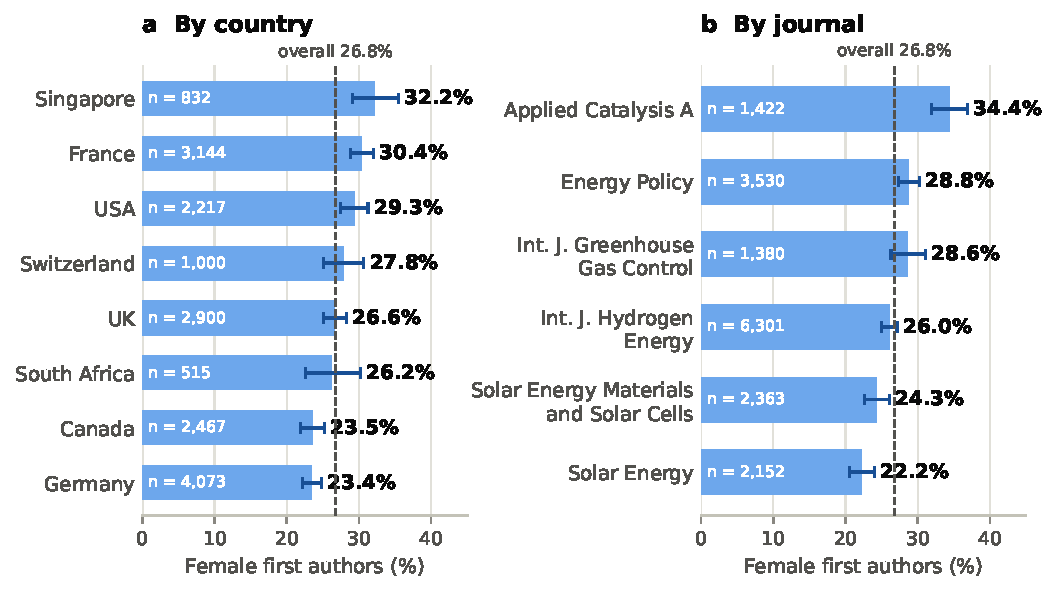
\includegraphics[width=\textwidth]{fig1_representation.pdf}
\caption{Share of female first authors by (a) country and (b) journal, with 95\% Wilson confidence intervals. The dashed line marks the overall share (26.8\%).}
\label{fig:representation}
\end{figure}

Because countries publish in different journals, differences between countries could simply reflect their research portfolios. They do not. In a logistic regression with both country and journal, the odds of a female first author relative to Germany remain higher in Singapore (odds ratio 1.58), France (1.40), the USA (1.30), Switzerland (1.28) and the UK (1.15; all $p<0.05$), while Canada (0.99) and South Africa (1.15) do not differ significantly from Germany. Relative to \textit{Solar Energy}, the odds are higher in \textit{Applied Catalysis A: General} (1.81), \textit{Energy Policy} (1.44), \textit{International Journal of Greenhouse Gas Control} (1.43) and \textit{International Journal of Hydrogen Energy} (1.27; all $p<0.001$). Country differences are also not the same in every journal (interaction $p<0.001$): for example, women are 37.9\% of first authors of Swiss articles in \textit{Energy Policy} but 16.0\% in \textit{Solar Energy}, and 41.8\% of first authors of French articles in \textit{Applied Catalysis A: General}.

\subsection{Temporal trends}

The female share of first authors was 26.6\% in 2010, fell to a low of 22.8\% in 2013 and reached 29.8\% in 2024 (Figure~\ref{fig:trend}). Over the complete years 2010-2024 the trend is positive and significant, consistent with H1c: the yearly share rises by 0.37 percentage points per year ($r=0.79$, $p<0.001$), and the article-level odds of a female first author increase by 2.0\% per year (odds ratio 1.020, $p<0.001$). The partial year 2025 (141 records, 20.6\% female) is excluded from trend estimation; including it in the year-level regression makes the trend non-significant ($r=0.31$, $p=0.25$), which illustrates how sensitive such summaries are to incomplete recent data. The trend remains positive and significant when low-confidence gender predictions are excluded ($+0.34$ points per year at a threshold of 0.6 and $+0.25$ at 0.7), when each article is counted once ($+0.34$), and when country and journal are controlled for (odds ratio 1.026 per year, $p<0.001$).

The rise is not uniform. Among journals it is strongest in \textit{Solar Energy}, where the female share rose from 15.9\% in 2010-2014 to 25.5\% in 2020-2024 ($+0.88$ points per year, $p<0.001$), and in \textit{Energy Policy} (25.4\% to 32.3\%; $+0.67$ points per year, $p=0.001$); the other four journals show smaller increases that are not clearly significant. The journal that started lowest has therefore risen fastest, which narrows the differences between journals. Among countries the rise is significant in the USA (24.3\% to 33.8\%), Germany (20.4\% to 27.2\%) and Canada (20.5\% to 26.6\%), while France is flat at about 30\%; trends differ between countries ($p=0.03$). The inflow of new authors shows the same direction: among authors appearing as first author for the first time in the dataset, the female share rose from 25.6\% in 2012 to 30.1\% in 2024 ($+0.42$ points per year, $p=0.005$).

\begin{figure}[htbp]
\centering
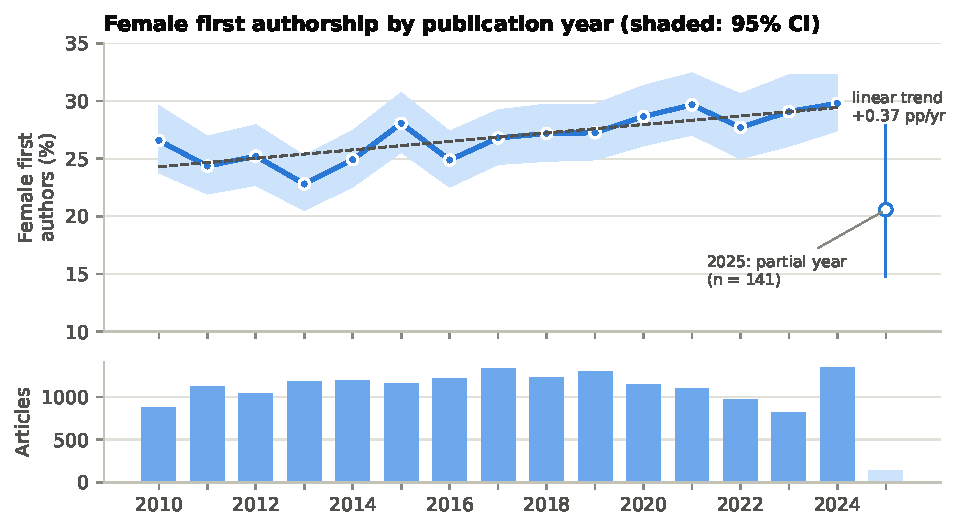
\includegraphics[width=\textwidth]{fig2_trend.pdf}
\caption{Female first authorship by publication year with 95\% confidence band (top) and number of article-country records per year (bottom). The dashed line is the 2010-2024 linear trend. 2025 is a partial year and is shown separately.}
\label{fig:trend}
\end{figure}

\subsection{Impact metrics}\label{sec:impact}

Table~\ref{tab:metrics} compares impact metrics by first-author gender. Male-first-authored articles receive 7.13\% more citations on average than female-first-authored articles (43.10 vs.\ 40.23). This is the raw gap expected under H3a, but the medians are almost identical (24 vs.\ 23) and the difference is not statistically significant (Mann-Whitney $p=0.10$). The gap in means therefore comes from a small number of very highly cited articles rather than from a difference for the typical article. Among the alternative metrics, captures, usage and social media show no significant gender difference, and mentions are marginally higher for female-first-authored articles ($p=0.04$). The clearest difference in Table~\ref{tab:metrics} is not in impact but in seniority: female first authors have markedly lower h-indices (mean 11.2 vs.\ 14.7; median 8 vs.\ 10; $p<0.001$).

\begin{table}[htbp]
\centering
\caption{Impact metrics and first-author h-index by first-author gender (article-country records). $p$-values are from two-sided Mann-Whitney U tests.}
\label{tab:metrics}
\begin{tabular}{lrrrrr}
\toprule
 & \multicolumn{2}{c}{Mean} & \multicolumn{2}{c}{Median} & \\
Metric & Male & Female & Male & Female & $p$ \\
\midrule
Citations (PlumX)    & 43.10 & 40.23 & 24 & 23 & 0.10 \\
Citations (Crossref) & 40.39 & 37.62 & 23 & 21 & 0.15 \\
Captures             & 72.02 & 69.50 & 41 & 41 & 0.51 \\
Mentions             & 0.34 & 0.39 & 0 & 0 & 0.04 \\
Usage                & 12.72 & 8.95 & 0 & 0 & 0.57 \\
Social media         & 250.44 & 204.25 & 0 & 0 & 0.64 \\
\midrule
First-author h-index & 14.71 & 11.21 & 10 & 8 & $<0.001$ \\
\bottomrule
\end{tabular}
\end{table}

Table~\ref{tab:models} and Figure~\ref{fig:citations} show how the citation difference changes as controls are added. In the log-linear models the unadjusted difference is $-2.3\%$ and not significant. After adjusting for publication year, journal and country it is $+1.9\%$, again not significant: female first authors are more common in recent years, when articles have had less time to be cited, and this accounts for the small raw gap. Consistent with H3b, no citation disadvantage remains once the context of publication is taken into account. After additionally adjusting for the first author's h-index, female-first-authored articles receive 6.0\% more citations ($p<0.001$). This last estimate depends on the specification: it is $+3.3\%$ ($p=0.20$) in the Poisson model and $+2.9\%$ ($p=0.21$) when gender predictions with confidence below 0.7 are excluded. It should also be read with care because the h-index is partly an outcome of past citations. The robust conclusion is that no adjusted specification shows a significant citation disadvantage for female-first-authored articles.

\begin{table}[htbp]
\centering
\caption{Difference in citations between female- and male-first-authored articles under increasing controls. Log-linear models are ordinary least squares on $\log(1+\text{citations})$; Poisson models are fitted to citation counts. $n = 17{,}148$.}
\label{tab:models}
\begin{tabular}{p{5.6cm}rrrrr}
\toprule
 & \multicolumn{3}{c}{Log-linear} & \multicolumn{2}{c}{Poisson} \\
Controls & Difference & 95\% CI & $p$ & Difference & $p$ \\
\midrule
M1: gender only & $-2.3\%$ & $-6.2$ to $+1.9$ & 0.28 & & \\
M2: + year, journal, country & $+1.9\%$ & $-1.3$ to $+5.3$ & 0.25 & $-3.1\%$ & 0.23 \\
M3: + first-author h-index & $+6.0\%$ & $+2.6$ to $+9.4$ & $<0.001$ & $+3.3\%$ & 0.20 \\
\bottomrule
\end{tabular}
\end{table}

\begin{figure}[htbp]
\centering
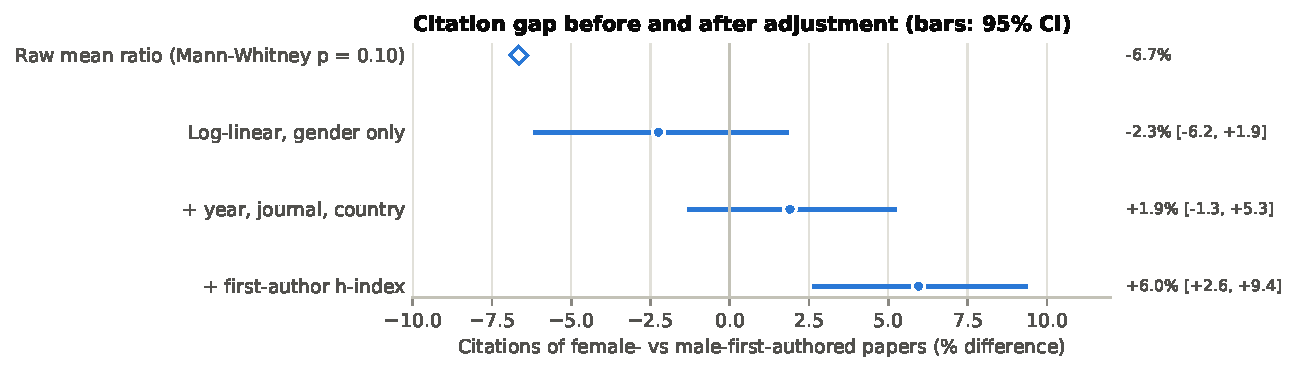
\includegraphics[width=0.9\textwidth]{fig3_citation_gap.pdf}
\caption{Citations of female- relative to male-first-authored papers. The diamond shows the raw ratio of means. Circles show estimates from log-linear models with progressively more controls, with 95\% confidence intervals (HC1 robust standard errors).}
\label{fig:citations}
\end{figure}

Two further checks support this conclusion. The raw gap is similar before and after 2020 (4.2\% for 2010-2019 and 4.8\% for 2020-2025; neither significant), so there is no sign that it has changed over time. And women are equally represented among highly cited articles: among the 13,602 unique articles published in 2010-2022, women are first authors of 25.7\% (95\% CI 23.5-28.1\%) of the 10\% most cited articles within their journal and year, against 26.4\% of all articles; 10.0\% of female-first-authored and 10.4\% of male-first-authored articles reach the top 10\% ($p=0.55$).

\subsection{Seniority, repeat authorship and collaboration}

The female share of first authors falls steadily with seniority, consistent with H4 (Figure~\ref{fig:seniority}a). Women are first authors of 30.6\% of articles whose first author has an h-index of 0-2 and 32.9\% at 3-5, but 25.4\% at 11-20, 20.9\% at 21-40 and 13.4\% above 40. In a logistic regression with year and journal controls, the odds of a female first author fall by 24\% per unit of $\log(1+\text{h-index})$ (odds ratio 0.76, $p<0.001$). The gradient is the same when each author is counted once and when gender predictions with confidence below 0.6 are excluded (28.4\% at an h-index of 0-2, falling to 9.9\% above 40). The difference between the most junior and the most senior first authors (17 percentage points) is larger than the difference between any two countries or journals.

Women are also less likely to appear repeatedly as first author. Of the 12,139 unique first authors, 28.1\% are women; 16.0\% of female first authors have two or more first-author articles in the dataset, against 19.6\% of male first authors ($p<0.001$). Women are 29.0\% of authors with a single first-author article, 24.6\% of those with two to four and 16.9\% of the 124 with five or more (Figure~\ref{fig:seniority}b). Because authors are matched by exact name, these figures are approximate.

Female-first-authored articles have slightly larger teams (mean 5.0 vs.\ 4.8 authors, $p<0.001$), and female first authors are less often the most senior member of the team: they have the highest h-index among the authors in 7.2\% of articles, against 11.6\% for male first authors. Women are under-represented among solo authors, at 19.1\% of the 728 solo-authored articles against 27.1\% of multi-authored ones. Most solo-authored articles are in \textit{Energy Policy}, where women are 23.7\% of solo authors and 29.8\% of first authors in teams. Adding team size and the highest co-author h-index to the citation model leaves the gender difference close to zero ($+1.1\%$, $p=0.53$).

\begin{figure}[htbp]
\centering
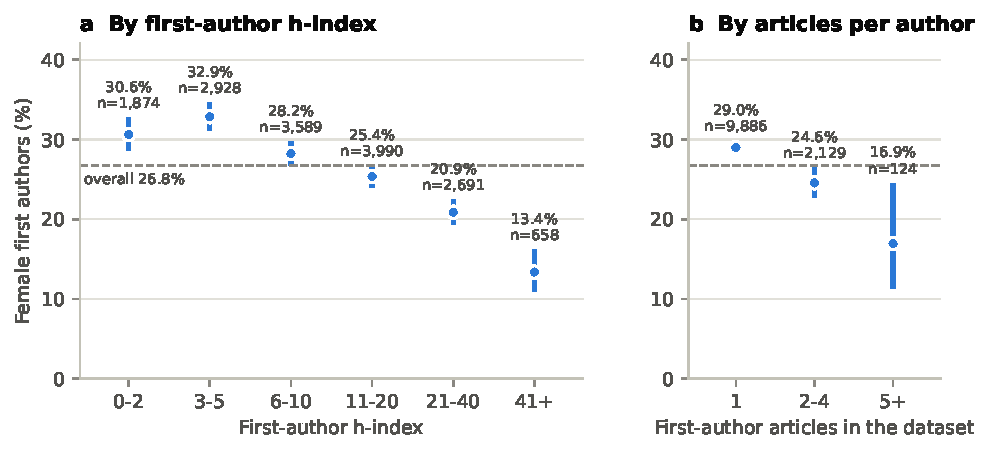
\includegraphics[width=\textwidth]{fig7_seniority.pdf}
\caption{Share of female first authors (a) by the first author's h-index, for unique articles, and (b) by the number of first-author articles an author has in the dataset, for unique authors. Bars are 95\% Wilson confidence intervals; the dashed line is the overall share.}
\label{fig:seniority}
\end{figure}

\subsection{Research focus by country and by gender}\label{sec:regional}

Research focus, proxied by journal, differs markedly by country (Figure~\ref{fig:journal_mix}). The \textit{International Journal of Hydrogen Energy} accounts for 55.9\% of Canadian, 51.1\% of South African and 44.6\% of French records. \textit{Solar Energy Materials and Solar Cells} is most prominent in Switzerland (29.5\%), Germany (21.1\%) and Singapore (17.8\%). \textit{Energy Policy} is a major outlet for the UK (30.6\%), Switzerland (27.2\%) and the USA (26.1\%).

\begin{figure}[htbp]
\centering
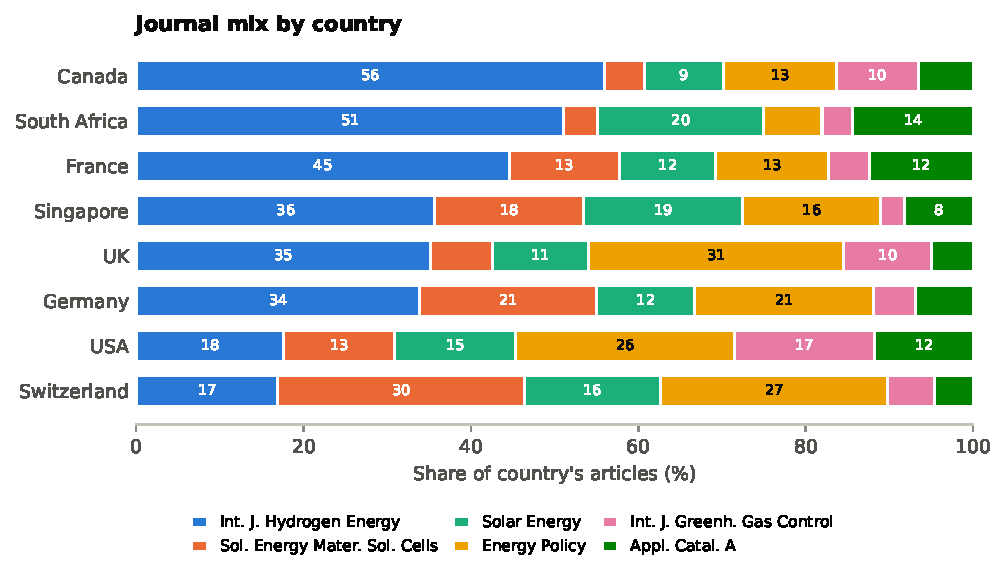
\includegraphics[width=\textwidth]{fig4_journal_mix.pdf}
\caption{Journal mix of each country's article-country records (\%). Segments under 8\% are unlabelled.}
\label{fig:journal_mix}
\end{figure}

Within journals, topics also differ by first-author gender (Table~\ref{tab:keywords}). Of the 134 author keywords used in at least 40 articles, 25 have a female share that differs significantly from the average, where about seven would be expected by chance. Keywords with the highest female share relate to electrochemistry and catalysis, biological hydrogen production and sustainability assessment; those with the lowest relate to silicon photovoltaics, wind power and simulation. This suggests that the differences between journals continue at a finer scale within them, although the numbers for individual keywords are small.

\begin{table}[htbp]
\centering
\caption{Author keywords with the highest and lowest share of female first authors, among keywords used in at least 40 unique articles. The overall share is 26.8\%.}
\label{tab:keywords}
\begin{tabular}{lrr@{\hskip 1.2cm}lrr}
\toprule
\multicolumn{3}{c}{Highest female share} & \multicolumn{3}{c}{Lowest female share} \\
Keyword & Articles & \% & Keyword & Articles & \% \\
\midrule
oxygen reduction reaction & 67 & 49.3 & silicon & 98 & 10.2 \\
electrocatalyst & 40 & 45.0 & wind power & 53 & 11.3 \\
dark fermentation & 56 & 44.6 & light trapping & 43 & 11.6 \\
heterogeneous catalysis & 51 & 43.1 & gas diffusion layer & 43 & 11.6 \\
life cycle assessment & 77 & 42.9 & simulation & 103 & 15.5 \\
energy transition & 111 & 41.4 & hydrogen safety & 80 & 16.2 \\
\bottomrule
\end{tabular}
\end{table}

Citations are distributed across countries roughly in proportion to output (Figure~\ref{fig:metric_share}). Germany and the UK together account for 40.1\% of citations (23.0\% and 17.1\%), in line with their shares of records (23.8\% and 16.9\%). Usage and social media counts are not comparable across countries. A non-zero usage value is recorded for 29.7\% of UK records but for only 1-3\% of records from the other countries; a single record holds 26.6\% of all usage, and five records hold 25.8\% of all social media counts. The UK's 81.8\% share of usage and Germany's 41.1\% share of social media therefore reflect data coverage and outliers, not readership or reach.

\begin{figure}[htbp]
\centering
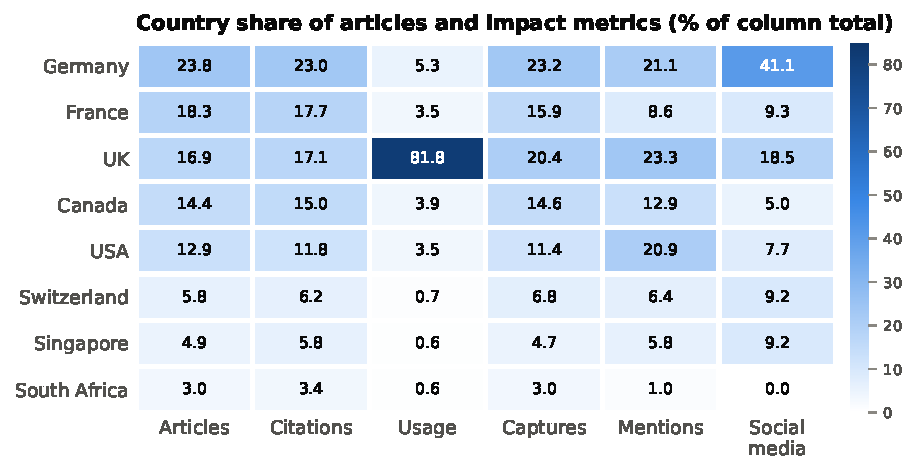
\includegraphics[width=0.9\textwidth]{fig5_metric_share.pdf}
\caption{Each country's share of total article-country records and of each impact metric (\% of column total). Usage and social media shares reflect uneven data coverage and a few outlying records and should not be interpreted as differences in reach.}
\label{fig:metric_share}
\end{figure}

\subsection{Sensitivity to gender-classification confidence}\label{sec:sensitivity}

The classifier is less confident for female-predicted first authors (mean probability 0.707) than for male-predicted ones (0.829). This holds even for unambiguous names: first authors named Sarah, Laura or Julia are all classified as female but with mean probabilities of 0.69-0.74, against 0.94-0.96 for Michael, Thomas or David. As a result, the estimated female share falls steeply as the minimum-confidence threshold rises: 26.8\% with no threshold, 24.5\% at 0.6, 17.2\% at 0.7, 9.5\% at 0.8 and 4.9\% at 0.9 (Figure~\ref{fig:threshold}). Thresholding therefore does not just remove noise; it systematically removes women. At the same time, the least confident predictions are close to guesses: among records with probability below 0.7, 46-48\% are labelled female, far above the overall share, so the unthresholded estimate is probably somewhat too high. We report unthresholded estimates and treat the absolute level of female representation as uncertain.

\begin{figure}[htbp]
\centering
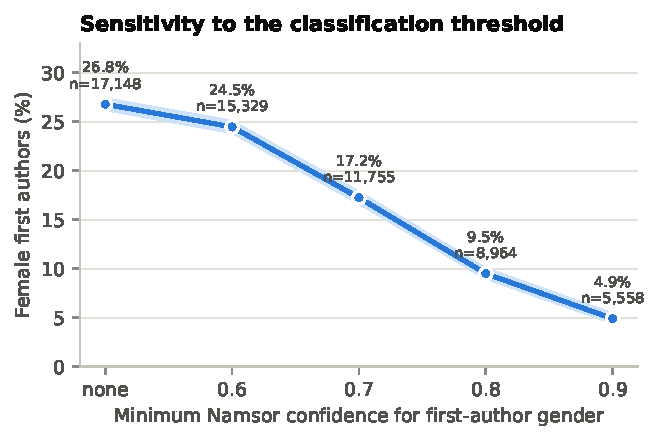
\includegraphics[width=0.7\textwidth]{fig6_threshold.pdf}
\caption{Share of female first authors among records retained at each minimum Namsor confidence, with 95\% confidence band; $n$ is the number of records retained.}
\label{fig:threshold}
\end{figure}

Comparisons between groups are affected to different degrees (Table~\ref{tab:threshold}). The ranking of journals is the same at thresholds of 0.6 and 0.7 as without a threshold, with \textit{Applied Catalysis A: General} highest and \textit{Solar Energy} lowest throughout, and the upward trend over time and the seniority gradient persist. The ranking of countries is less stable. France is among the highest and Canada the lowest at every threshold, but Singapore falls from the highest share (32.2\%) to the second lowest (15.4\%) at a threshold of 0.7, where only 40\% of its records are retained, compared with 57-79\% for the other countries. Singapore's position, and to a lesser extent the ordering of the other countries, should therefore be treated as uncertain \note{validate the classifier against a hand-labelled sample, stratified by country}.

\begin{table}[htbp]
\centering
\caption{Share of female first authors (\%) by country and journal at different minimum classifier probabilities, and the share of each group's records retained at 0.7.}
\label{tab:threshold}
\begin{tabular}{lrrrr}
\toprule
 & No threshold & $\geq 0.6$ & $\geq 0.7$ & Retained at 0.7 (\%) \\
\midrule
Singapore    & 32.2 & 27.7 & 15.4 & 40 \\
France       & 30.4 & 29.1 & 23.6 & 72 \\
USA          & 29.3 & 25.9 & 16.6 & 64 \\
Switzerland  & 27.8 & 26.5 & 20.4 & 76 \\
UK           & 26.6 & 24.2 & 15.8 & 66 \\
South Africa & 26.2 & 20.5 & 15.6 & 57 \\
Canada       & 23.5 & 19.7 & 11.9 & 63 \\
Germany      & 23.4 & 22.6 & 16.1 & 79 \\
\midrule
Applied Catalysis A: General & 34.4 & 31.6 & 26.4 & 63 \\
Energy Policy & 28.8 & 27.7 & 19.7 & 76 \\
Int. J. Greenhouse Gas Control & 28.6 & 26.5 & 19.5 & 71 \\
Int. J. Hydrogen Energy & 26.0 & 23.1 & 15.7 & 64 \\
Solar Energy Materials and Solar Cells & 24.3 & 22.9 & 15.7 & 70 \\
Solar Energy & 22.2 & 18.5 & 11.8 & 68 \\
\bottomrule
\end{tabular}
\end{table}

%===========================================================
\section{Discussion}
%===========================================================

We discuss the results in the order of the research questions and then turn to their implications.

\subsection{Representation: persistent but slowly narrowing under-representation}

The first research question asked what share of first authors are women and how it varies. At 26.8\%, female first authorship in these energy journals remains well below parity, in every country and every journal (H1a). The figure is higher than the share of fewer than one in six reported for energy journals in 1999-2013 \citep{Sovacool2014}, although the two studies differ in journals, period and in counting all authors rather than first authors.

Differences between journals are larger and more robust than differences between countries (H1b). The ordering of journals, with catalysis highest, policy in the middle and solar energy lowest, is stable under every check we applied and is consistent with the gender composition of the disciplines the journals draw on, chemistry having a higher share of women than physics or electrical engineering. Differences between countries remain after accounting for journal mix, so they are not explained by national research portfolios. They may reflect national policies supporting women in science and engineering, educational pipelines or academic career structures \note{support with references}. However, the ordering of countries, and Singapore's position in particular, depends on the gender classifier (Section~\ref{sec:sensitivity}), so we do not draw conclusions from the ranking of individual countries.

The share is rising (H1c), by about 0.37 percentage points per year. At this rate parity would be several decades away if the trend continued linearly, in line with projections for related fields \citep{Holman2018}. The rise is concentrated in particular journals and countries. \textit{Solar Energy} started from the lowest share and has risen fastest, and the USA, Germany and Canada have risen while France, which started highest, has not. The picture is therefore one of convergence from different starting points rather than of uniform progress.

\subsection{Research focus: countries and genders specialise}

The second research question concerned research focus. National research portfolios differ, with hydrogen research dominating in Canada, South Africa and France, solar materials research prominent in Switzerland and Germany, and energy policy a larger share of output in the UK, Switzerland and the USA. These patterns are likely to reflect national energy strategies, industrial structure and funding priorities \note{support with references, or treat as a hypothesis}. Within journals, the keywords associated with female first authors differ from those associated with male first authors, which suggests that the division between fields with more and fewer women continues at the level of topics. This finding is exploratory, and a fuller analysis would apply topic modelling to titles and abstracts, as in the UK phase of the project.

\subsection{Impact: no evidence of a citation penalty}

The third research question asked whether impact differs by gender. The raw citation advantage of male-first-authored articles (7.13\%) is small and not statistically significant, and it does not survive adjustment for publication year, journal and country (H3a, H3b). Women are equally represented among the most highly cited articles, and the gap has not changed over time. Once the first author's h-index is also taken into account, female-first-authored articles receive slightly more citations in our main specification, although the size and significance of this advantage depend on the model, and the h-index is itself partly an outcome of past citation. We therefore conclude that there is no evidence of a citation penalty for women in these journals, and we do not claim an advantage. This is consistent with career-level studies that find equal impact for the same body of work \citep{Huang2020}, and differs from studies that report a citation gap in aggregate data \citep{Lariviere2013}.

Citations are distributed across countries in proportion to their output, so we find no concentration of impact beyond research volume. The apparent concentration of usage and social media activity in particular countries reflects uneven data coverage and a few outlying records, which is a warning against using alternative metrics for comparisons between countries without checking their coverage.

\subsection{Seniority and progression: where the gap is largest}

The fourth research question concerned seniority. The steepest gradient in our data is not between countries or journals but along seniority (H4). Women are close to a third of the most junior first authors and about one in eight of the most senior, they are less likely to publish repeatedly as first author, and they are less often the most senior member of their team. Together with the absence of a citation penalty, this points to retention and progression rather than the reception of women's work as the main source of inequality, in line with evidence that career length and drop-out explain most of the gender gap in research careers \citep{Huang2020}.

These are cross-sectional patterns. A lower female share among senior authors partly reflects the lower share of women entering the field in earlier decades, and our data cannot separate this cohort effect from attrition. The rising female share among new first authors suggests that the inflow is improving, although slowly.

\subsection{Methodological implications}

The sensitivity analysis shows that choices about classification confidence can change estimates of female representation by more than a factor of five, and can reorder countries. Excluding low-confidence predictions is not a neutral precaution, because the classifier is less confident for female names, including common ones. Bibliometric equity studies that rely on name-based inference should report the classifier, its confidence distribution by predicted gender and the sensitivity of each main result to the threshold, and should be cautious in comparing groups whose names differ in how well they are classified \citep{Santamaria2018,Lockhart2023}. In our data, comparisons between journals, over time and by seniority are robust to this choice, whereas the absolute level of representation and the ranking of countries are not.

%===========================================================
\section{Conclusions}
%===========================================================

\subsection{What we learnt}

Across six energy journals and eight countries, women are about a quarter of first authors. They are a minority in every country and journal, with larger differences between research fields than between countries. Their share is rising by about a third of a percentage point per year, fastest where it started lowest. Articles with a female first author are cited as much as those with a male first author once the year, journal and country of publication are taken into account, and women are equally represented among the most highly cited articles. The largest gap is in seniority: the female share falls from about a third of the most junior first authors to about an eighth of the most senior, and women are less likely to publish repeatedly as first author. The main inequality in these data is therefore in participation and progression, not in recognition.

\subsection{Limitations and what we did not learn}

The first group of limitations concerns gender inference. Gender is inferred from names as a binary category; this may misclassify individuals, performs unequally across name origins and does not capture non-binary identities. As a result, the study does not establish the true level of female representation, which is probably somewhat below the 26.8\% we report, and it does not establish a reliable ranking of countries. It also says nothing about the gender of co-authors, about collaboration networks or about last and corresponding authors, because co-author gender could not be inferred reliably. The analysis covers first authors only, and authorship-order conventions differ between fields.

The second group concerns seniority. The h-index is measured at the time of data collection and is an imperfect proxy for seniority, and authors are identified by name in the analysis of repeat authorship. The study cannot say why women are fewer among senior authors, in particular how much is due to women leaving research and how much to smaller cohorts of women in the past.

The third group concerns scope and data. The sample is limited to six journals from one publisher and eight countries, most of them high-income, so the results should not be generalised to energy research as a whole or to other regions. Countries are defined by author affiliation, not nationality, and articles with authors in several study countries are counted under each. Recent articles have had less time to accumulate citations, and 2025 is incomplete. Usage and social media metrics are not comparable across countries in these data.

Finally, the study is observational. It cannot establish causes, and it cannot explain the differences between countries and fields, which would require qualitative evidence.

\subsection{Future work}

The most important next step is to validate the gender predictions against a hand-labelled sample stratified by country, or against a second inference method, and to correct the estimates accordingly. Further work should use Scopus author identifiers and career start years to follow cohorts of authors over time, which would separate attrition from cohort effects; extend the analysis to last and corresponding authors; add journals covering wind, nuclear and storage research, and countries with emerging research systems; and revisit the topic-modelling and language analyses from the project's UK phase on the multi-country dataset. Qualitative research with energy researchers would help explain the patterns observed here.

%-----------------------------------------------------------
\section*{Acknowledgements}
%-----------------------------------------------------------
This work was supported by the IGNITE Network+ and Imperial College London.

%-----------------------------------------------------------
\section*{Data availability}
%-----------------------------------------------------------
The analysis code is available at \note{repository URL}. The processed article-level data are derived from Elsevier, Scopus, Crossref and Namsor services and will be shared subject to those providers' terms of use \note{confirm what can be shared}.

%-----------------------------------------------------------
\section*{Declaration of competing interest}
%-----------------------------------------------------------
\note{The authors declare that they have no known competing financial interests or personal relationships that could have appeared to influence the work reported in this paper.}

%-----------------------------------------------------------
\begin{thebibliography}{00}

\bibitem{UNESCO2017}
UNESCO, 2017.
Cracking the Code: Girls' and Women's Education in Science, Technology, Engineering and Mathematics (STEM).
UNESCO Publishing, Paris.

\bibitem{Elsevier2020}
Elsevier, 2020.
The Researcher Journey Through a Gender Lens: An Examination of Research Participation, Career Progression and Perceptions Across the Globe.
Elsevier, Amsterdam.

\bibitem{Pearl-Martinez2016}
Pearl-Martinez, R., Stephens, J.C., 2016.
Toward a gender diverse workforce in the renewable energy transition.
Sustainability: Science, Practice and Policy 12(1), 8-15.
\url{https://doi.org/10.1080/15487733.2016.11908149}

\bibitem{IRENA2019}
IRENA, 2019.
Renewable Energy: A Gender Perspective.
International Renewable Energy Agency, Abu Dhabi.
Available at: \url{https://www.irena.org/publications/2019/Jan/Renewable-Energy-A-Gender-Perspective}

\bibitem{Lariviere2013}
Larivi\`ere, V., Ni, C., Gingras, Y., Cronin, B., Sugimoto, C.R., 2013.
Global gender disparities in science.
Nature 504(7479), 211-213.
\url{https://doi.org/10.1038/504211a}

\bibitem{Holman2018}
Holman, L., Stuart-Fox, D., Hauser, C.E., 2018.
The gender gap in science: How long until women are equally represented?
PLOS Biology 16(4), e2004956.
\url{https://doi.org/10.1371/journal.pbio.2004956}

\bibitem{West2013}
West, J.D., Jacquet, J., King, M.M., Correll, S.J., Bergstrom, C.T., 2013.
The role of gender in scholarly authorship.
PLOS ONE 8(7), e66212.
\url{https://doi.org/10.1371/journal.pone.0066212}

\bibitem{Huang2020}
Huang, J., Gates, A.J., Sinatra, R., Barab\'asi, A.-L., 2020.
Historical comparison of gender inequality in scientific careers across countries and disciplines.
Proceedings of the National Academy of Sciences 117(9), 4609-4616.
\url{https://doi.org/10.1073/pnas.1914221117}

\bibitem{Sovacool2014}
Sovacool, B.K., 2014.
What are we doing here? Analyzing fifteen years of energy scholarship and proposing a social science research agenda.
Energy Research \& Social Science 1, 1-29.
\url{https://doi.org/10.1016/j.erss.2014.02.003}

\bibitem{Santamaria2018}
Santamar\'ia, L., Mihaljevi\'c, H., 2018.
Comparison and benchmark of name-to-gender inference services.
PeerJ Computer Science 4, e156.
\url{https://doi.org/10.7717/peerj-cs.156}

\bibitem{Lockhart2023}
Lockhart, J.W., King, M.M., Munsch, C., 2023.
Name-based demographic inference and the unequal distribution of misrecognition.
Nature Human Behaviour 7(7), 1084-1095.
\url{https://doi.org/10.1038/s41562-023-01587-9}

\bibitem{Carroll2023}
Carroll, P., Singh, B., Mangina, E., 2023.
Uncovering gender dimensions in energy policy using natural language processing.
SSRN preprint.
\url{https://papers.ssrn.com/sol3/papers.cfm?abstract_id=4427707}

\bibitem{Hirsch2005}
Hirsch, J.E., 2005.
An index to quantify an individual's scientific research output.
Proceedings of the National Academy of Sciences 102(46), 16569-16572.
\url{https://doi.org/10.1073/pnas.0507655102}

\bibitem{Wilson1927}
Wilson, E.B., 1927.
Probable inference, the law of succession, and statistical inference.
Journal of the American Statistical Association 22(158), 209-212.

\bibitem{MannWhitney1947}
Mann, H.B., Whitney, D.R., 1947.
On a test of whether one of two random variables is stochastically larger than the other.
Annals of Mathematical Statistics 18(1), 50-60.

\bibitem{Namsor2024}
Namsor, 2024.
Namsor API: Gender, Origin, and Ethnicity Inference from Names.
Available at: \url{https://namsor.app/}
(accessed 15 January 2025).

\end{thebibliography}

\end{document}
